\chapter{RTS AI: \textit{StarCraft: Broodwar}}
\newglossaryentry{micro}{name=micro-management,description={gameplay actions that are manually addressed by the player; the way of maximizing one's army efficiency by using the units to the maximum of their potential.}}

\begin{quotation}\textit{
We think of life as a journey with a destination (success, heaven). But we missed the point. It was a musical thing, we were supposed to sing and dance while music was being played.}\\
\begin{flushright}Alan Watts\end{flushright}
\end{quotation}

\lettrine{T}{his} chapter explains the basics of RTS gameplay, particularly StarCraft. We then list the (computational) challenges brought by RTS gameplay. We present a transversal decomposition of the RTS AI domain in levels of abstractions (strategy, tactics, \glos{micro}), which we will use for the rest of the dissertation.

\chaptertoc

\section{How does the game work}

\subsection{RTS Gameplay}
We first introduce the basic components of a real-time strategy (RTS) game. The player is usually referred as the ``commander'' and perceives the world in an allocentric ``God's view'', performing mouse and keyboard actions to give orders to units (or squads of units) within a circumvented area (the ``map''). In a RTS, players need to gather resources to build military units and defeat their opponents. To that end, they often have \textit{worker units} (or extraction structures) than can gather resources needed to build \textit{workers}, \textit{buildings}, \textit{military units} and \textit{research upgrades}. Workers are often also builders (as in StarCraft) and are weak in fights compared to military units. Resources may have different uses, for instance in StarCraft: minerals are used for everything, whereas gas is only required for advanced buildings or military units, and technology upgrades. Buildings and research upgrades define technology trees (directed acyclic graphs) and each state of a 
\newglossaryentry{techtree}{name={tech tree},description={abbreviation for ``technological tree'', state of the technology (buildings, researches, upgrades) which are unlocked/available to a given player.}}
%\newglossaryentry{techtree}{name={tech tree},description={abbr. for ``technological tree'', the state of buildings and technologies evolution (technologies which are unlocked) of a given player}}
\glos{techtree} (or \newglossaryentry{buildtree}{name={build tree},description={abbrev. for ``buildings tree'', state of the buildings (and thus production) unlocked by a player}}\glos{buildtree}) allow for different unit type production abilities and unit spells/abilities. The military units can be of different types, any combinations of ranged, casters, contact attack, zone attacks, big, small, slow, fast, invisible, flying... In the end, a central part of the gameplay is that units can have attacks and defenses that counter each others as in a soft rock-paper-scissors. Also, from a player point of view, most RTS games are only partially observable due to the \textit{\glos{fogofwar}} which hides units and new buildings which are not in sight range of the player's units. 


In chronological order, RTS include (but are not limited to): Ancient Art of War, Herzog Zwei, Dune II, Warcraft, Command \& Conquer, Warcraft II, C\&C: Red Alert, Total Annihilation, Age of Empires, StarCraft, Age of Empires II, Tzar, Cossacks, Homeworld, Battle Realms, Ground Control, Spring Engine games, Warcraft III, Total War, Warhammer 40k, Sins of a Solar Empire, Supreme Commander, StarCraft II. The differences in gameplay are in the order of number, nature and gathering methods of resources; along with construction, research and production mechanics. The duration of games vary from 15 minutes for the fastest to (1-3) hours for the ones with the biggest maps and longest gameplays. We will now focus on StarCraft, on which our robotic player is implemented.


\subsection{A StarCraft Game}
\textit{StarCraft} is a science-fiction RTS game released by Blizzard Entertainment$^{TM}$ in March 1998. It was quickly expanded into \textit{StarCraft: Brood War} (SC: BW) in November 1998. In the following, when referring to StarCraft, we mean StarCraft with the Brood War expansion. StarCraft is a canonical RTS game in the sense that it helped define the genre and most gameplay mechanics seen in other RTS games are present in StarCraft. It is as much based on strategy than tactics, by opposition to the Age of Empires and Total Annihilation series in which strategy is prevalent. In the following of the thesis, we will focus on duel mode, also known as 1 vs. 1 (1v1). Team-play (2v2 and higher) and ``free for all'' are very interesting but were not studied in the framework of this research. These game modes particularly add a layer of coordination and bluff respectively.


StarCraft sold 9.5 millions licenses worldwide, 4.5 millions in South Korea alone \citep{StarCraftNumbers}, and reigned on competitive RTS tournaments for more than a decade. Numerous international competitions (World Cyber Games, Electronic Sports World Cup, BlizzCon, OnGameNet StarLeague, MBCGame StarLeague) and professional gaming (mainly in South Korea \citep{Chee05}) produced a massive amount of data of highly skilled human players. In South Korea, there are two TV channels dedicated to broadcasting competitive video games, particularly StarCraft. The average salary of a \glos{pro-gamer} there was up to 4 times the average South Korean salary \citep{MYMPGM} (up to \$200,000/year on contract for NaDa). Professional gamers perform about 300 actions (mouse and keyboard clicks) per minute while following and adapting their strategies, while their hearts reach 160 beats per minute (BPM are displayed live in some tournaments). StarCraft II is currently (2012) taking over StarCraft in competitive gaming but a) there is still a strong pool of highly skilled StarCraft players and b) StarCraft II has a really similar gameplay.


StarCraft (like most RTS) has a \textit{\glos{replay}} mechanism, which enables to record every player's actions such that the state of the game can be deterministically re-simulated. The only piece of stochasticity comes from ``attack miss rates'' ($\approx 47\%$) when a unit is on a lower ground than its target. These randomness generator seed is saved along with the actions in the replay. All high level players use this feature heavily either to improve their play or study opponents' styles. Observing replays allows player to see what happened under the \textit{\glos{fogofwar}}, so that they can understand timing of technologies and attacks, and find clues/evidences leading to infer the strategy as well as weak points.


In StarCraft, there are three factions with very different units and technology trees:
\begin{itemize}
    \item \textit{Terran}: humans with strong defensive capabilities and balanced, averagely priced biological and mechanical units.
    \item \textit{Protoss}: advanced psionic aliens with expensive, slow to produce but resistant units.
    \item \textit{Zerg}: insectoid alien race with cheap, quick to produce but weak units.
\end{itemize}

All factions use workers to gather resources, and all other characteristics are different: from military units to ``\gloss{techtree}'', gameplay styles. Races are so different that highly skilled players focus on playing with a single race (but against all three others). There are two types of resources, often located close together, minerals and gas. From minerals, one can build basic buildings and units, which opens the path to more advanced buildings, technologies and units, which will in turn all require gas to be produced. While minerals can be gathered at an increasing rate (bounded asymptotically) the more workers are put at work, the gas gathering rate is quickly limited to 3 workers per gas geyser (i.e. per base). There is another third type of ``special'' resource (called \newglossaryentry{supply}{name=supply,description={maximum number of units that a player can control at a given time, can be increased up to a hard limit (200 in StarCraft).}}\textit{\glos{supply}}), which is the current limit of population a player can control. It can be upgraded by building special buildings (Protoss Pylon, Terran Supply Depot) or units (Zerg Overlord), giving 9 to 10 additional supply, up to a hard limit of 200. Some units cost more supply than others (from 0.5 for a Zergling to 8 for a Protoss Carrier or Terran Battlecruiser). In Figure~\ref{fig:SC_eco}, we show the very basics of Protoss economy and buildings. %In Figure~\ref{fig:SC_battle}, we show

\newglossaryentry{mini-map}{name=mini-map,description={radar view of the full game area, shown in the bottom corner of the interface in StarCraft.}}
\begin{figure}[!ht]
\begin{center}
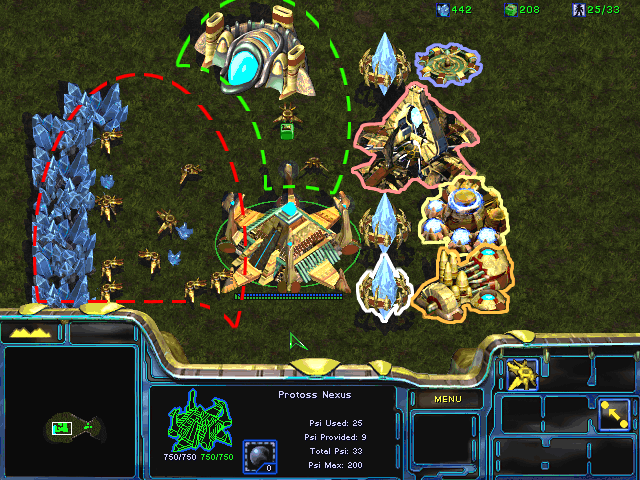
\includegraphics[width=13cm]{images/SC_eco.png}
\caption{A StarCraft screenshot of a Protoss base, with annotations. The interface (heads up display at the bottom) shows the \textit{\glos{mini-map}}. The center of the interface (bottom) shows the selected unit (or group of units), here the Protoss Nexus (main economical building, producing workers and to which resources are brought) which is in the center of the screen and circled in green. The bottom right part shows the possible actions (here build a Protoss Probe or set a rally point). The top right of the screen shows the minerals (442), gas (208) and \glos{supply} (25 total on 33 current maximum). The dotted lines demarcate economical parts with active workers: red for minerals mining and green for gas gathering. The plain cut outs of buildings show: a Pylon (white), a Forge (orange, for upgrades and access to static defense), a Cybernetics Core (yellow, for technological upgrades and expanding the tech tree), a Gateway (pink, producing ground units), a Photon Cannon (blue, static defense).}
\label{fig:SC_eco}
\end{center}
\end{figure}

\newglossaryentry{opening}{name=opening,description={in Chess as in RTS games: the first strategic moves of the game, the strategy of the early game},plural=openings}
\newglossaryentry{buildorder}{name=build order,description={a formal specification of timings (most often indexed on total population count) at which to perform build actions in the early game.}}
To reach a competitive amateur level, players have to study \textit{\gloss{opening}} and hone their \textit{\gloss{buildorder}}. An opening corresponds to the first strategic moves of a game, as in other abstract strategy games (Chess, Go). They are classified/labeled with names from high level players. A build-order is a formally described and accurately timed sequence of buildings to construct in the beginning. As there is a bijection between optimal population and time (in the beginning, before any fight), build orders are indexed on the total population of the player as in the example for Protoss in table~\ref{bo:two_gates_goon_range}. 
At the highest levels of play, StarCraft games usually last between 6 (shortest games, with a successful rush from one of the player) to 30 minutes (long economically and technologically developed game).
%%%\begin{verbatim}
%%%population-thing to build
%%%8-Pylon 
%%%10-Gateway 
%%%12-Gas Assimilator
%%%13-Make Zealot Once Gateway completes 
%%%16-Pylon 
%%%18-Core
%%%20-Make Zealot 
%%%22-Pylon, make Dragoon
%%%27-Start Dragoon Range Upgrade, Pylon 
%%%30-Robotics Facility, Gateway
%%%32-Pylon 
%%%37-Make Shuttle, Start cutting Probes (don't make probes anymore for now) 
%%%39-Observatory, Then Robotic Support Bay
%%%43-make observer 
%%%44-Pylon 
%%%48-Make Reaver 
%%%52-Pylon, Start Back Probe Production (make probes again) 
%%%\end{verbatim}
\begin{table}[ht]
\begin{center}
\begin{tabular}{|l|l|l|}
\hline
Supply & Build & Note \\
\hline
8 & Pylon & ``supply/psi/control/population'' building \\
10 & Gateway & units producing structure \\
12 & Assimilator & constructed on a gas geyser, to gather gas \\
14 & Cybernetics Core & technological building \\
16 & Pylon & ``supply/psi/control/population'' building \\
16 & Range & it is a research/tech \\
16 & Dragoon & first military unit \\
\hline
\end{tabular}
\end{center}
\caption{An example of the beginning of a ``2 Gates Goon Range'' Protoss build order which focus on building dragoons and their attack range upgrade quickly.}
\label{bo:two_gates_goon_range}
\end{table}

%``Cutting'' workers (here, Probes for Protoss) production is a common feat of highly optimized ``timing attacks'' builds.
\begin{figure}[!ht]
\begin{center}
\begin{tabular}{cc}
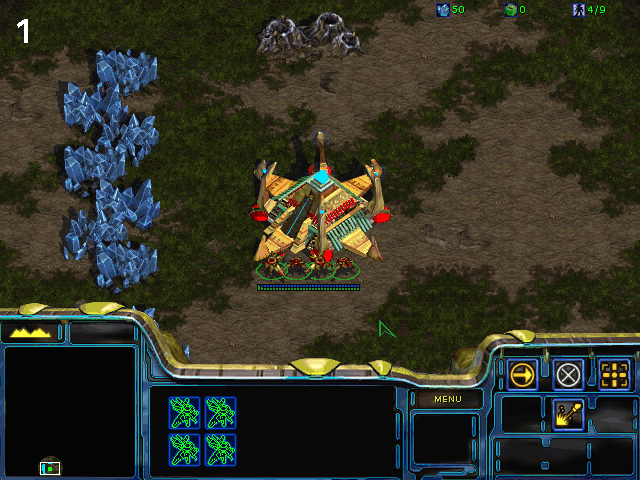
\includegraphics[width=7.8cm]{images/SC_game/SC_start_game.png} &
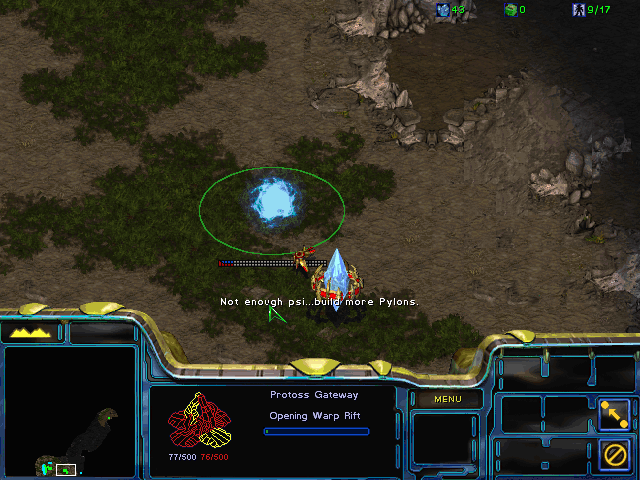
\includegraphics[width=7.8cm]{images/SC_game/SC_first_gate.png} \\
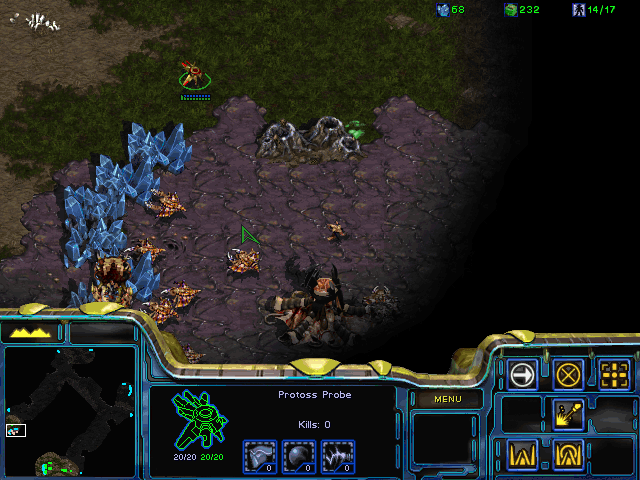
\includegraphics[width=7.8cm]{images/SC_game/SC_scout_opponent.png} & 
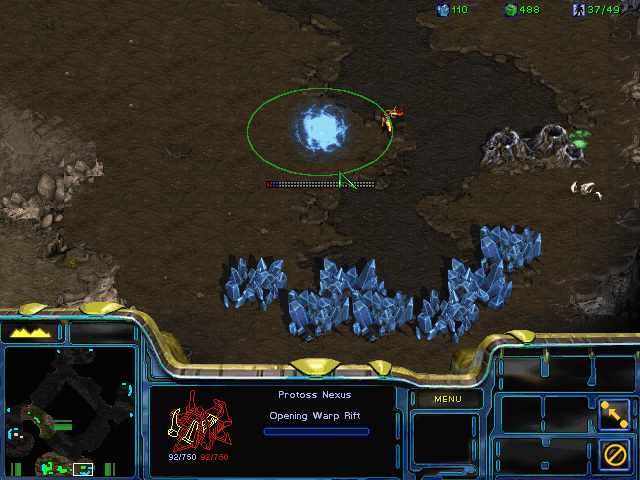
\includegraphics[width=7.8cm]{images/SC_game/SC_expand.png} \\ 
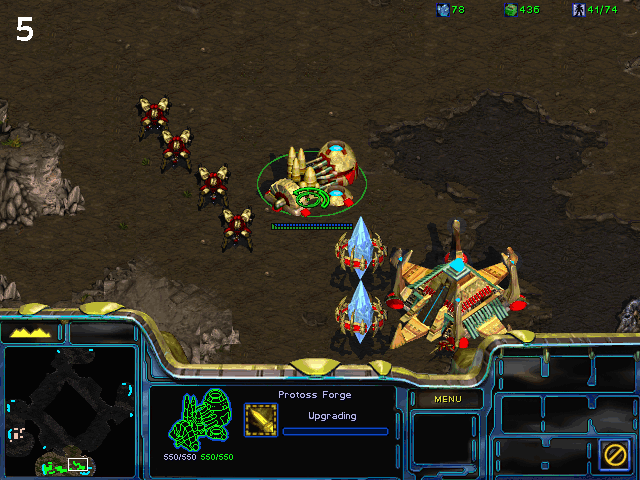
\includegraphics[width=7.8cm]{images/SC_game/SC_upgrade_attack.png} & 
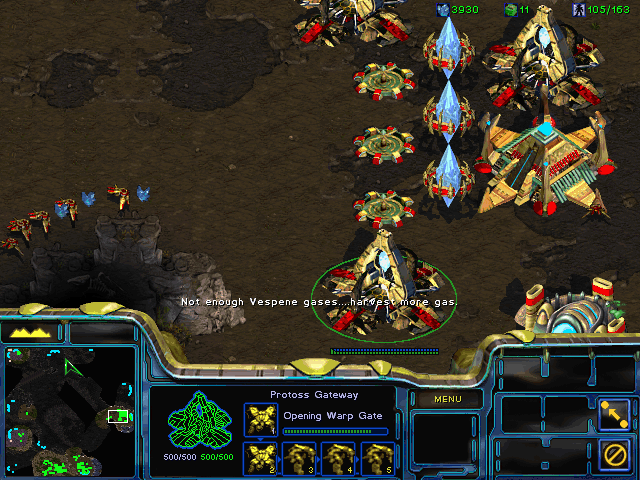
\includegraphics[width=7.8cm]{images/SC_game/SC_queue_production.png}
\end{tabular}
%SC_first_pylon.png
\caption{Start and economical parts of a StarCraft game. The order of the screenshots goes from left to right and from top to bottom.}
\label{fig:SC_game1}
\end{center}
\end{figure}

\begin{figure}[!ht]
\begin{center}
\begin{tabular}{cc}
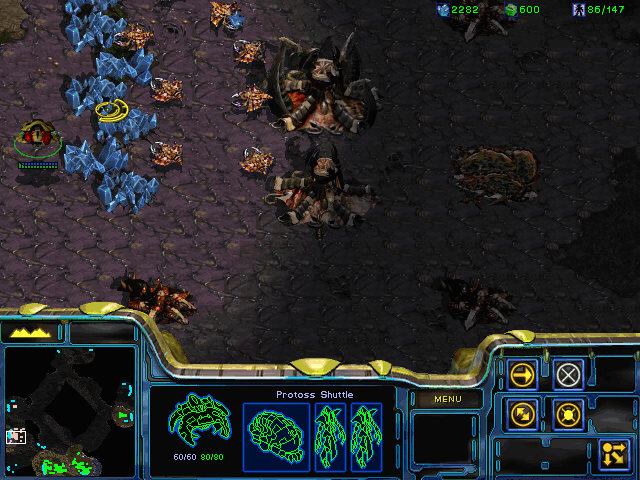
\includegraphics[width=7.8cm]{images/SC_game/SC_drop2a.png} &
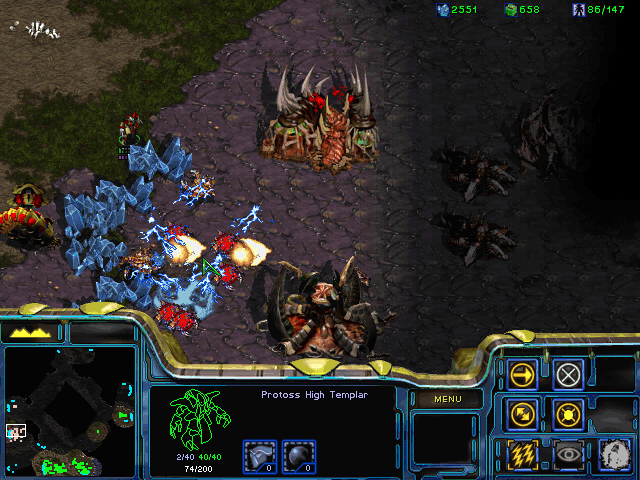
\includegraphics[width=7.8cm]{images/SC_game/SC_drop2b.png} \\
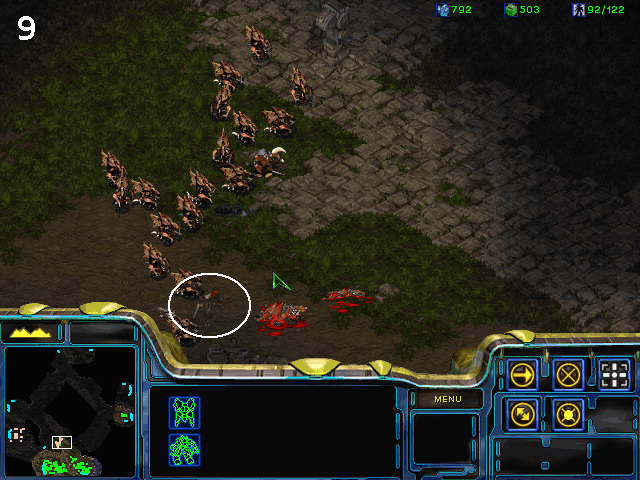
\includegraphics[width=7.8cm]{images/SC_game/SC_dt_army.png} & 
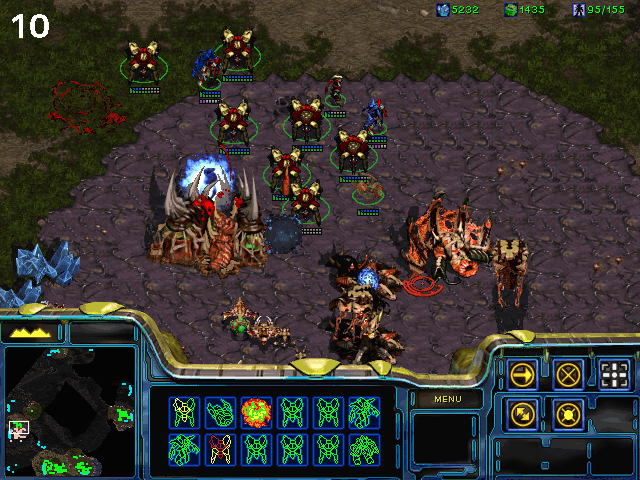
\includegraphics[width=7.8cm]{images/SC_game/SC_final_attack.png}
\end{tabular}
\caption{Military moves from a StarCraft (PvT) game. The order of the screenshots goes from left to right and from top to bottom.}
\label{fig:SC_game2}
\end{center}
\end{figure}

We now present the evolution of a game (Figures~\ref{fig:SC_game1} and \ref{fig:SC_game2}) during which we tried to follow the build order presented in table~\ref{bo:two_gates_goon_range} (``2 Gates Goon Range''\footnote{On Teamliquid: \url{http://wiki.teamliquid.net/starcraft/2_Gate_Goon_Range_(vs._Terran)}}) but we had to adapt to the fact that the opponent was Zerg (possibility for a faster rush) by building a Gateway at 9 supply and building a Zealot (ground contact unit) before the first Dragoon. The first screenshot (image 1 in Figure~\ref{fig:SC_game1}) is at the very start of the game: 4 Probes (Protoss workers), and one Nexus (Protoss main building, producing workers and depot point for resources). At this point players have to think about what \gloss{opening} they will use. Should we be aggressive early on or opt for a more defensive opening? Should we specialize our army for focused tactics, to the detriment of being able to handle situations (tactics and armies compositions) from the opponent that we did not foresee? In picture 2 in the same Figure (\ref{fig:SC_game1}), the first gate is being built. At this moment, players often send a worker to ``scout'' the enemy's base, as they cannot have military units yet, it is a safe way to discover where they are and inquiry about what they are doing. In picture 3, the player scouts their opponent, thus gathering the first bits of information about %their race (which is known beforehand if not playing against ``Random'') and 
their early tech tree. Thus, knowing to be safe from an early attack (``rush''), the player decides to go for a defensive and economical strategy for now. Picture 4 shows the player ``expanding'', which is the act of making another base at a new resource location, for economical purposes. In picture 5, we can see the upgrading of the ground weapons along with 4 ranged military units, staying in defense at the expansion. This is a technological decision of losing a little of potential ``quick military power'' (from military units which could have been produced for this minerals and gas) in exchange of global upgrade for all units (alive and to be produced), for the whole game. This is an investment in both resources and time. Picture 6 showcases the production queue of a Gateway as well as workers transferring to a second expansion (third base). Being safe and having expanded his \glos{techtree} to a point where the army composition is well-rounded, the player opted for a strategy to win by profiting from an economical lead. Figure~\ref{fig:SC_game2} shows the aggressive moves of the same player: in picture 7, we can see a flying transport with artillery and area of effect ``casters'' in it. The goal of such an attack is not to win the game right away but to weaken the enemy's economy: each lost worker has to be produced, and, mainly, the missing gathering time adds up quite quickly. In picture 8, the transport in unloaded directly inside the enemy's base, causing huge damages to their economy (killing workers, Zerg Drones). This is the use of a specialized tactics, which can change the course of a game. At the same time, it involves only few units (a flying transport and its cargo), allowing for the main army to stay in defense at base. It capitalizes on the maneuverability of the flying Protoss Shuttle, the technological advancements allowing area of effects attacks and the large zone that the opponent has to cover to defend against it. In picture 9, an invisible attacking unit (circled in white) is harassing the oblivious enemy's army. This is an example of how technology advance on the opponent can be game changing (the opponent does not have detection in range, thus is vulnerable to cloaked units). Finally, picture 10 shows the final attack, with a full ground army marching on the enemy's base.


\section{RTS AI Challenges}
In combinatorial game theory terms, competitive StarCraft (1 versus 1) is a zero sum, partial-information, deterministic\footnote{The only stochasticity is in attacks failures (miss rate) from lower grounds to higher grounds, which is easily averaged.} strategy game. 
StarCraft subsumes Wargus (Warcraft II open source clone), which has an estimated mean branching factor $1.5.10^3$ \citep{LTW} (Chess: $\approx 35$, Go: $<360$): \cite{bgweberPhD} finds a branching factor greater than $1.10^6$ for StarCraft. In a given game (with maximum map size) the number of possible positions is roughly of $10^{11500}$, versus the Shannon number for Chess ($10^{43}$) \citep{Shannon_1950}. Also, we believe strategies are much more balanced in StarCraft than in most other games. Otherwise, how could it be that more than a decade of professional gaming on StarCraft did not converge to a finite set of fixed (imbalanced) strategies?

Humans deal with this complexity by abstracting away strategy from low level actions: there are some highly restrictive constraints on where it is efficient (``optimal'') to place economical main buildings (Protoss Nexus, Terran Command Center, Zerg Hatchery/Lair/Hive) close to minerals spots and gas geysers. Low-level \glos{micro} decisions have high \textit{horizontal continuity} and humans see these tasks more like playing a musical instrument skillfully. Finally, the continuum of strategies is analyzed by players and some distinct strategies are identified as some kinds of ``invariants'', or ``entry points'' or ``principal components''. From there, strategic decisions impose some (sometimes hard) constraints on the possible tactics, and the complexity is broken by considering only the interesting state space due to this high \textit{vertical continuity}.

Most challenges of RTS games have been identified by \citep{Buro03,Buro04callfor}. We will try to anchor them in the human reasoning that goes on while playing a StarCraft game.
\begin{itemize}
    \item \textit{Adversarial planning under uncertainty} (along with \textit{resource management}): it diverges from traditional planning under uncertainty in the fact that the player also has to plan \textit{against} the opponent's strategy, tactics, and actions. From the human point of view, he has to plan for which buildings to build to follow a chosen \glos{opening} and subsequent strategies, under a restricted resources (and time) budget. At a lower level, and less obvious for humans, are the plans they make to coordinate units movements.
    \item \textit{Learning and opponent modeling}, Buro accurately points out that human players need very few (``a couple of'') games to spot their opponents' weaknesses. Somehow, human opponent modeling is related to the ``induction scandal'', as Russell called it: how do humans learn so much so fast? We learn from our mistakes, we learn the ``play style'' of our opponent's, we are quickly able to ask ourselves: ``what should I do now given what I have seen \textit{and} the fact that I am playing against player XYZ?''. ``Could they make the same attack as last time?''. To this end, we use high level representations of the states and the actions with compressed invariants, causes and effects.
    \item \textit{Spatial and temporal reasoning} (along with \textit{decision making under uncertainty}), this is related to planning under uncertainty but focuses on the special relations between what can and what cannot be done in a given time. Sadly, it was true in 2004 but is still true today: ``RTS game AI [...] falls victim to simple common-sense reasoning''. Humans learn sequences of actions, and reason only about actions coherent with common sense. For AI of complex systems, this common-sense is hard to encode and to use.
    %\item Resource management
    %\item Decision making under uncertainty
    \item Collaboration (teamplay), which we will not deal with here: a lot has to do with efficient communication and ``teammate modeling''.
\end{itemize}
As we have seen previously more generally for multi-player video games, all these challenges can be handled by Bayesian modeling. %The Cox-Jaynes theorem particularly comes to mind from ``induction scandal'' 
While acknowledging these challenges for RTS AI, we now propose a different task decomposition, in which different tasks will solve some parts of these problems at their respective levels.

% TODO ?


\section{Tasks decomposition and linking}
\begin{figure}[!ht]
\begin{center}
\begin{small}
\begin{tikzpicture}
  \path[mindmap,concept color=black!80!white,text=white]
    node[concept] {RTS AI: predict, decide, perform}
    [clockwise from=-30]
    child[concept color=orange!90!black] {
      node[concept] {Micro}
      child[concept color=red!80!magenta] { node[concept] {React} }
      child { node[concept] {Optimize} }
      child[concept color=blue!30!cyan] { node[concept] {Cooperate} }
    }
    child[concept color=blue!95!black] { % TODO change color
      node[concept] {Tactics}
      child[concept color=red!80!magenta] { node[concept] {When?} }
      child { node[concept] {Where?} }
      child[concept color=blue!30!cyan] { node[concept] {How?} }
    }
    child[concept color=green!70!black] {
      node[concept] {Strategy}
      child[concept color=red!80!magenta] { node[concept] {Economy}} %{Initiative} }
      child { node[concept] {Army}} %{Army composition} }
      child[concept color=blue!30!cyan] { node[concept] {Technology}} %{Spendings balance} }
    };  
\end{tikzpicture}
\end{small}
\end{center}
\caption{A mind-map of RTS AI. This is the tasks decomposition that we will use for the rest of the thesis.}
\label{fig:mindmapRTS}
\end{figure}

We decided to decompose RTS AI in the three levels which are used by the gamers to describe the games: \textit{strategy}, \textit{tactics}, \textit{micro-management}. We remind the reader that parts of the map not in the sight range of the player's units are under \textit{\glos{fogofwar}}, so the player has only partial information about the enemy buildings and army. The way by which we expand the tech tree, the specific units composing the army, and the general stance (aggressive or defensive) form what we call \textit{strategy}. At the lower level, the actions performed by the player (human or not) to optimize the effectiveness of its units is called \textit{\glos{micro}}. In between lies \textit{tactics}: where to attack, and how. A good human player takes much data in consideration when choosing: are there flaws in the defense? Which spot is more worthy to attack? How much am I vulnerable for attacking here? Is the terrain (height, chokes) to my advantage? The concept of strategy is a little more abstract: at the beginning of the game, it is closely tied to the build order and the intention of the first few moves and is called the \textit{opening}, as in Chess. Then, the long term strategy can be partially summed up by three signals/indicators:
\begin{itemize}
    \item aggression: how much is the player aggressive or defensive?
    \item initiative: how much is the player adapting to the opponent's strategy vs. how much is the player being original?
    \item technology/production/economy (tech/army/eco) distribution of resources: how much is the player spending (relatively) in these three domains?
\end{itemize}
\newglossaryentry{expand}{name=expand,description={either placement of a new base or the action to take a new base (to collect more resources).}}
At high levels of play, the tech/army/eco balance is putting a hard constraint on the aggression and initiative directions: if a player invested heavily in their army production, they should attack soon to leverage this investment. To the contrary, all other things being equal, when a player \gloss{expand}, they are being weak until the expansion repaid itself, so they should play defensively. Finally, there are some technologies (researches or upgrades) which unlocks an ``attack timing'' or ``attack window'', for instance when a player unlocks an invisible technology (or unit) before that the opponent has detection technology (detectors). On the other hand, while ``teching'' (researching technologies or expanding the \glos{techtree}), particularly when there are many intermediate technological steps, the player is vulnerable because of the immediate investment they made, which did not pay off yet.

From this RTS domain tasks decomposition, we can draw the mind map given in Figure~\ref{fig:mindmapRTS}. We also characterized these levels of abstractions by:
\begin{itemize}
    \item the conditioning that the decisions on one abstraction level have on the other, as discussed above: strategy conditions tactics which conditions low-level actions (that does not mean than there cannot be some feedback going up the hierarchy).
    \item the quantity of direct information that a player can hope to get on the choices of their opponent. While a player can see directly the micro-management of their enemy (movements of units on the battlefront), they cannot observe all the tactics, and a big part of tactics gameplay is to hide or fake them well. Moreover, key technological buildings are sometimes hidden, and the player has to form beliefs about the long term strategy of the opponent (without being in their head).
    \item the time which is required to switch behaviors of a given level. For instance a change of strategy will require to either \textit{a)} (technology) build at least two buildings or a building and a research/upgrade, \textit{b)} (army) build a few units, \textit{c)} take a new expansion (new base). A change of tactics corresponds to a large repositioning of the army(ies), while a change in micro-management is very quick (like moving units out of an area-of-effect damage zone).
\end{itemize}
This is shown in Figure~\ref{fig:sc_abstraction_times}. We will discuss the state of the art for the each of these subproblems (and the challenges listed above) in their respective parts.

\begin{figure}[htp]
\centerline{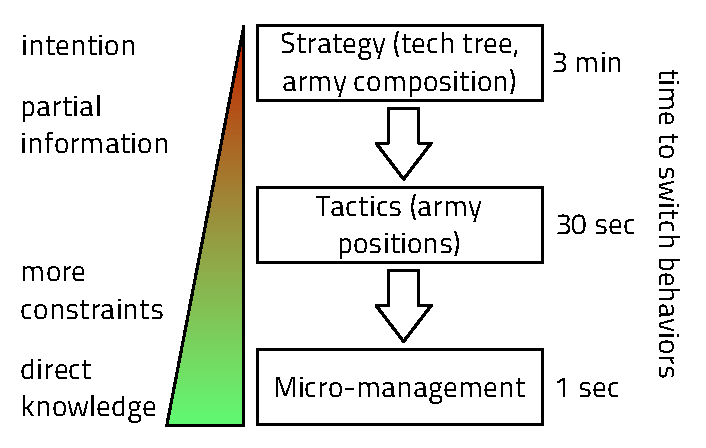
\includegraphics[width=7cm]{images/starcraft_levels_abstraction_light.pdf}}
\caption{Gameplay levels of abstraction for RTS games, compared with their level of direct (and complete) information and orders of magnitudes of time to chance their policies.}
\label{fig:sc_abstraction_times}
\end{figure}


To conclude, we will now present our works on these domains (strategy, tactics, micro-management) in separate chapters. In Figure~\ref{fig:conceptbbq}, we present the flow of informations between the different inference and decision-making parts of the bot architecture. One can also view this problem as having a good model of one's strategy, one's opponent strategy, and taking decisions. The software architecture that we propose is to have services building and maintaining the model of the enemy as well as our state, and decision-making modules using all this information to give orders to actuators (filled in gray in Fig.~\ref{fig:conceptbbq}).

\begin{figure}[!ht]
\begin{center}
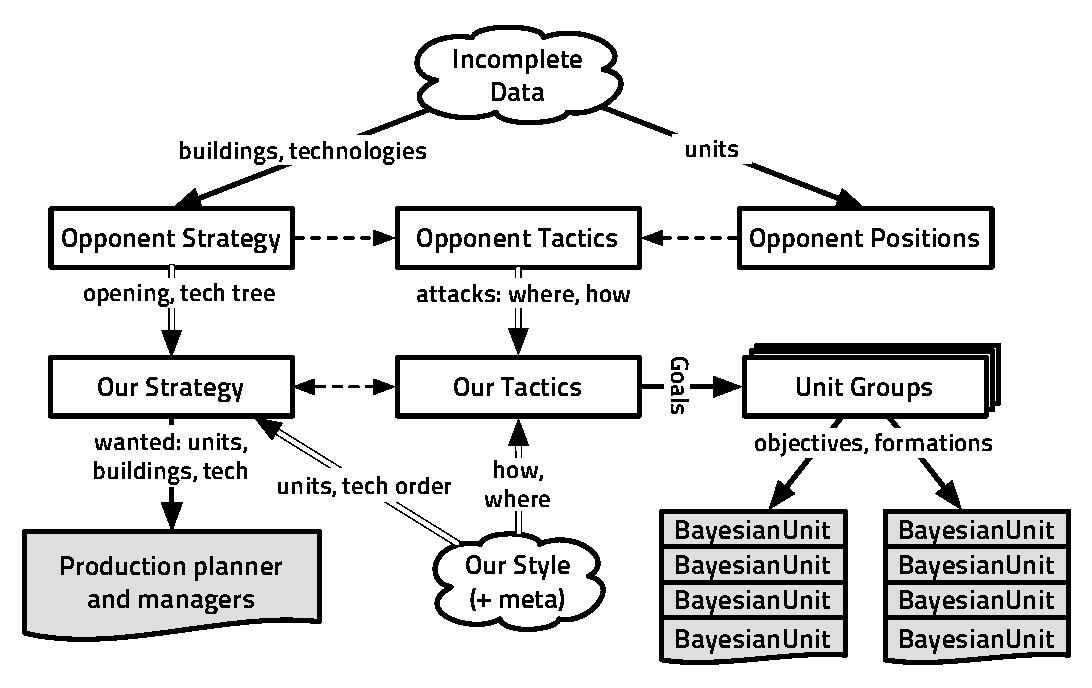
\includegraphics[width=13cm]{images/starcraft_bbq_concept.pdf}
\end{center}
\caption{Information-centric view of the architecture of the major components of the bot. Arrows are labeled with the information or orders they convey: dotted arrows are conveying constraints, double lined arrows convey distributions, plain and simple arrows convey direct information or orders. The gray parts perform game actions (as the physical actions of the player on the keyboard and mouse).}
\label{fig:conceptbbq}
\end{figure}


